\subsubsection{monolith::component::BaseComponent}

\label{monolith::component::BaseComponent}
\begin{figure}[H]
	\centering
	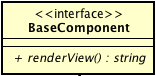
\includegraphics[scale=0.5]{Sezioni/SottosezioniST/img/BaseComponent.png}
	\caption{monolith::component::BaseComponent}
\end{figure}

\begin{itemize}
\item \textbf{Descrizione:} Interfaccia base che rappresenta un qualsiasi oggetto che può essere inserito all'interno di un bolla.
\item \textbf{Utilizzo:} Interfaccia che viene implementata ogni qualvolta uno sviluppatore intende definire una nuova tipologia di componente che è possibile inserire all'interno di una bolla.
\item \textbf{Attributi:}
\item \textbf{Metodi:}
\begin{itemize}
\item \textit{public renderView():string}\\
Genera il codice HTML, CSS e JavaScript necessario per visualizzare il componente.
\end{itemize}
\end{itemize}